\documentclass[a4paper,10pt]{article}

\usepackage{amssymb}
\usepackage{amsmath}
\usepackage{graphicx}
\usepackage{subfigure}

\title{Finite Volume experiments on convection/diffusion equations}
\author{Eivind Fonn}
\date{\today}

\begin{document}

\maketitle

\abstract{This document details numerical experiments on the Finite Volume
code for convection/diffusion equations in the LehrFEM library.}

\section{Experiment 1}

\[-\epsilon\Delta u + u_x = 1\]

The above equation will be solved on the triangle
$\Omega = \{(x,y)\;|\;0\leq x\leq1,\;-x\leq y\leq x\}$. As can be readily verified,
a solution to this equation is

\[ u(x,y) = x - \frac{1}{1-e^{-1/\epsilon}}\left(e^{-(1-x)/\epsilon}-e^{-1/\epsilon}\right). \]

We will use prescribed Dirichlet boundary conditions on the whole of $\partial\Omega$, to get
the above solution.

As $\epsilon\to0$ the problem will become convection-dominated, and there will be a boundary layer
at $x=1$. We will investigate the discretization errors as $\epsilon\to0$ and $h\to0$, where
$h$ is the meshwidth.

\begin{figure}[!ht]
\centering
\subfigure{\includegraphics[width=5cm]{e1_sol_h6_e4_top.eps}}
\subfigure{\includegraphics[width=5cm]{e1_sol_h6_e4.eps}}
\caption{Numerical solution for $\epsilon=10^{-3}$, $h=3.7\cdot10^{-3}$.}
\end{figure}

\begin{figure}[!ht]
\centering
\subfigure{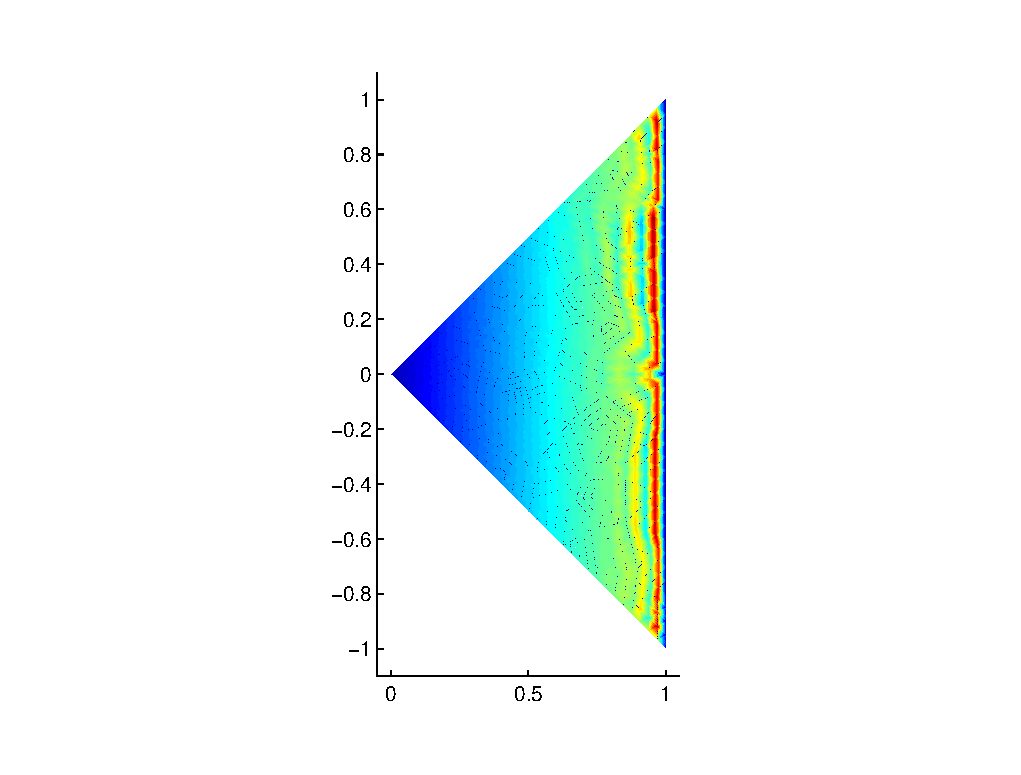
\includegraphics[width=5cm]{e1_sol_h2_e4_bdlosc_top.eps}}
\subfigure{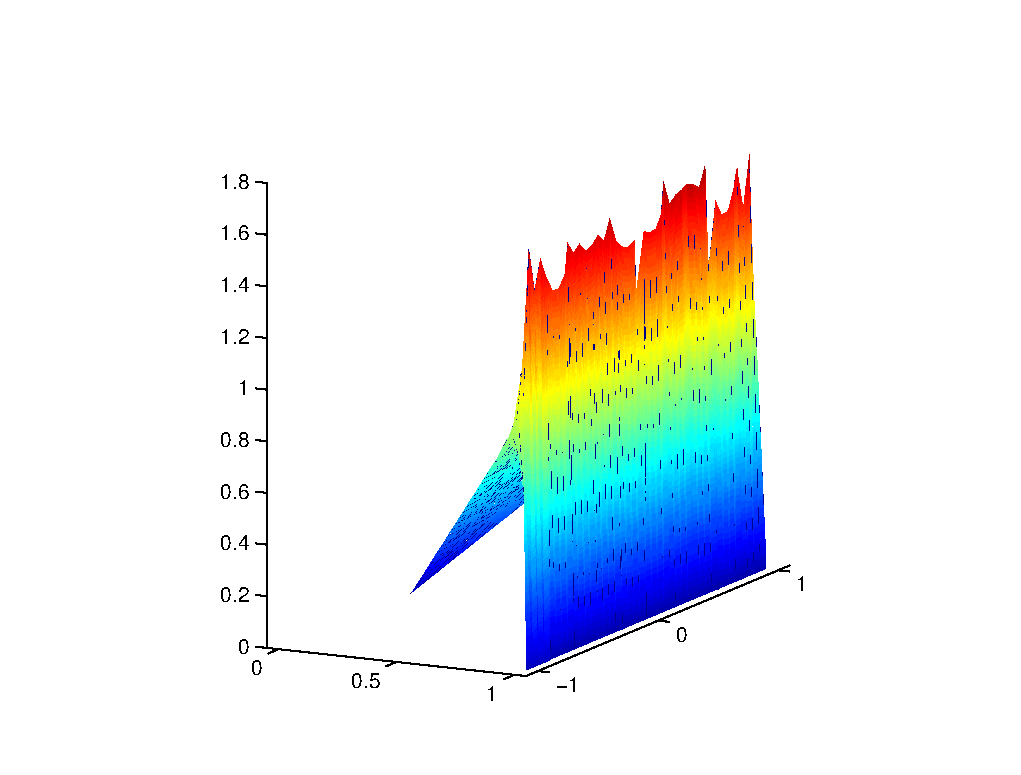
\includegraphics[width=5cm]{e1_sol_h2_e4_bdlosc.eps}}
\caption{Numerical solution for $\epsilon=10^{-3}$, $h=6\cdot10^{-2}$. Note the boundary
    layer oscillations.}
\end{figure}

\begin{figure}[!ht]
\centering
\subfigure{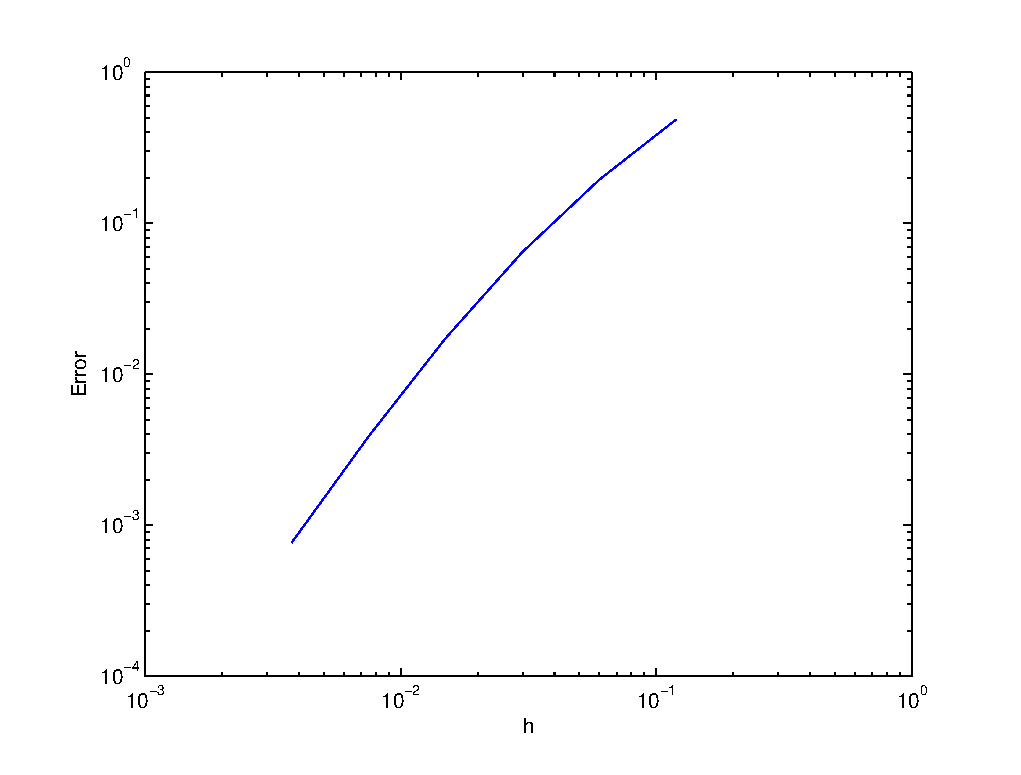
\includegraphics[width=5cm]{e1_l1err_vs_h.eps}}
\subfigure{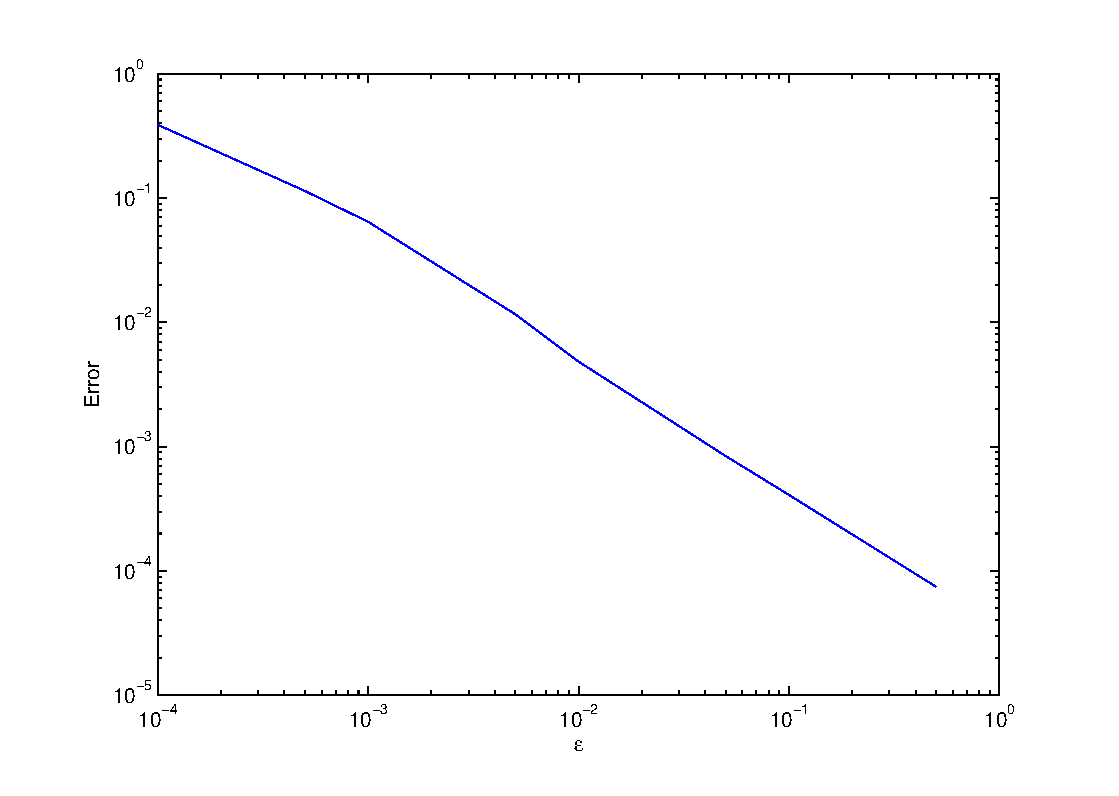
\includegraphics[width=5cm]{e1_l1err_vs_eps.eps}}
\caption{Discretization error measured in L1-norm, dependence on $h$ and $\epsilon$.}
\end{figure}

\begin{figure}[!ht]
\centering
\subfigure{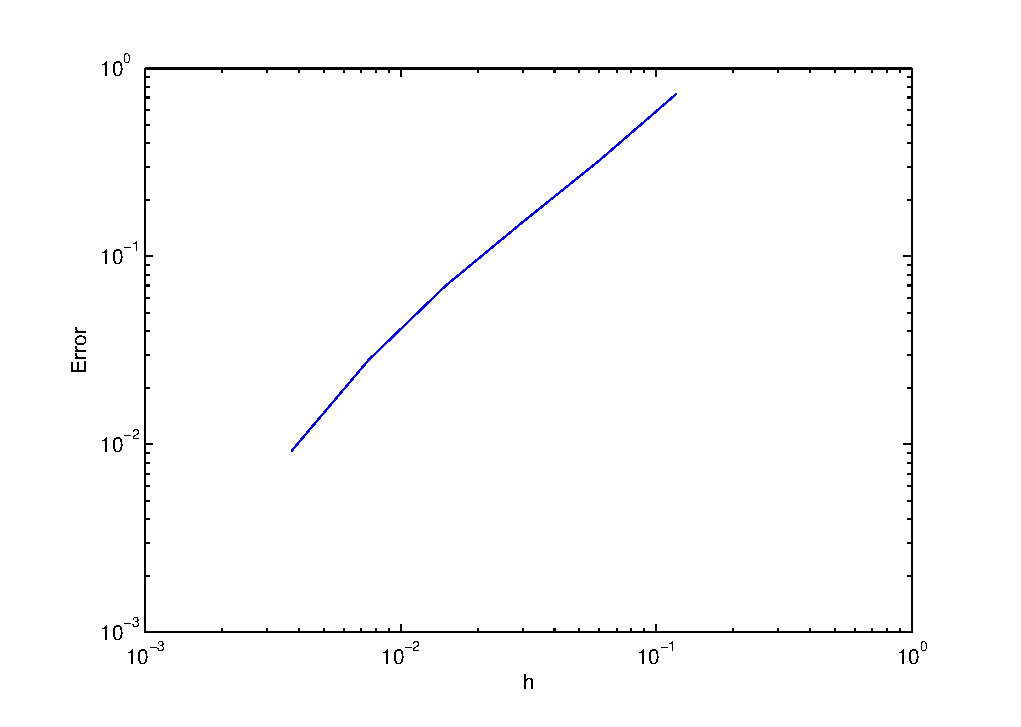
\includegraphics[width=5cm]{e1_l2err_vs_h.eps}}
\subfigure{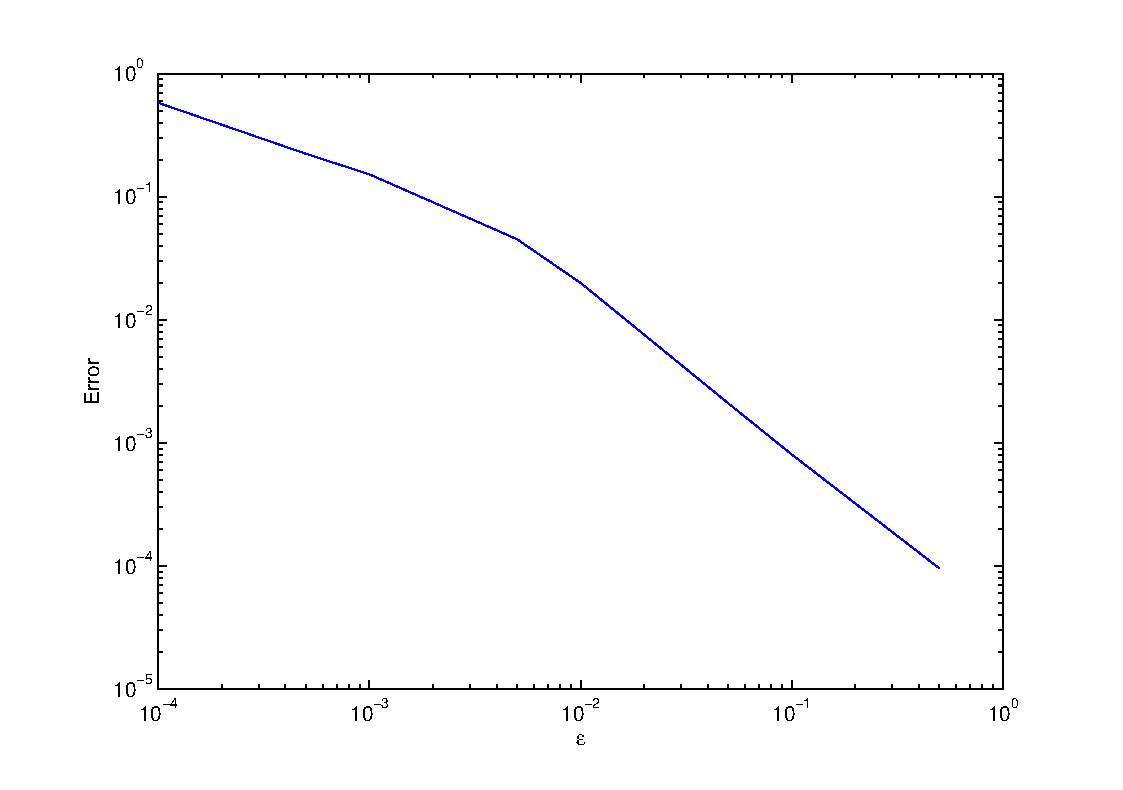
\includegraphics[width=5cm]{e1_l2err_vs_eps.eps}}
\caption{Discretization error measured in L2-norm, dependence on $h$ and $\epsilon$.}
\end{figure}

\begin{figure}[!ht]
\centering
\subfigure{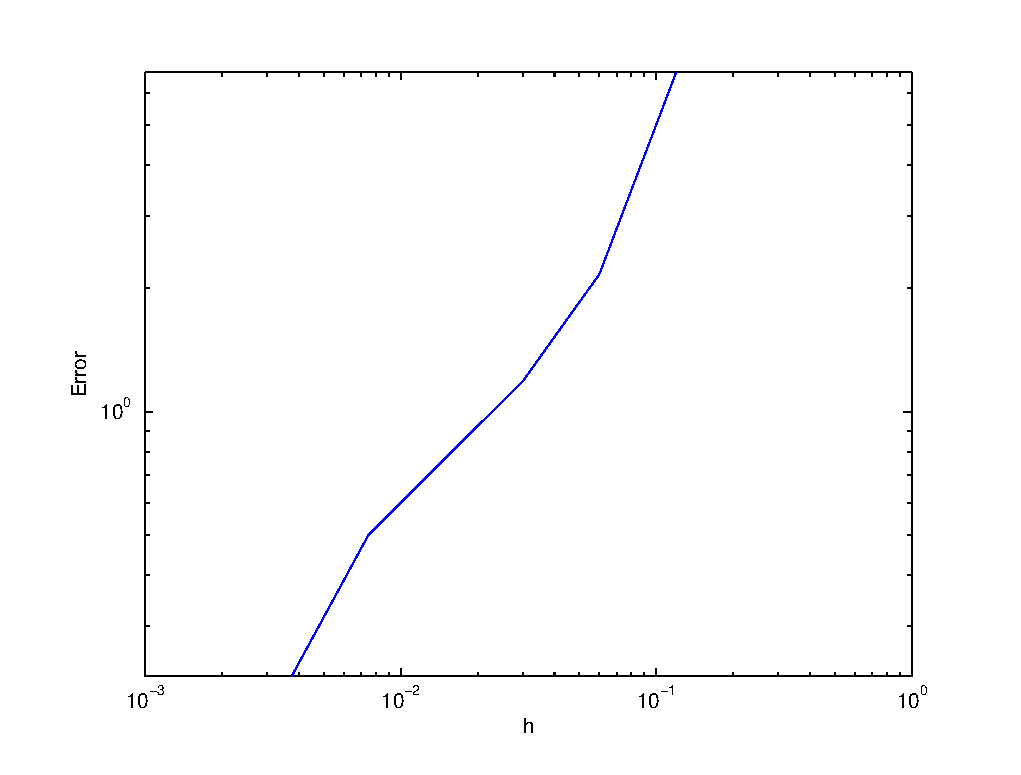
\includegraphics[width=5cm]{e1_linferr_vs_h.eps}}
\subfigure{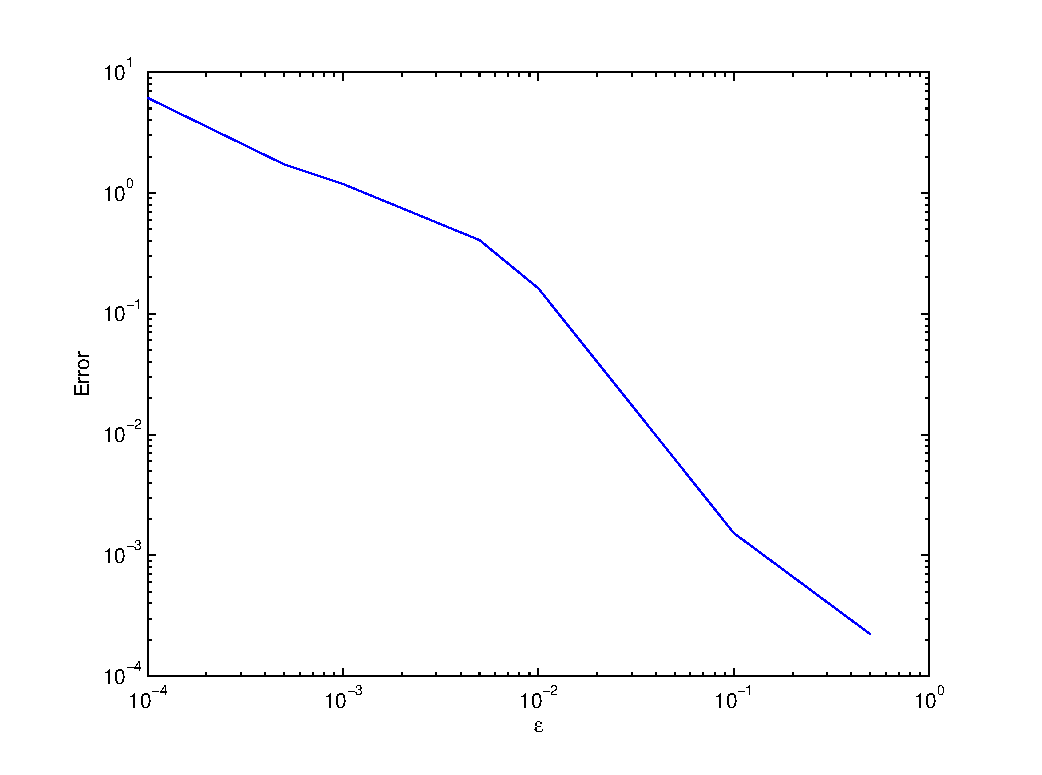
\includegraphics[width=5cm]{e1_linferr_vs_eps.eps}}
\caption{Discretization error measured in the $\infty$-norm, dependence on $h$ and $\epsilon$.}
\end{figure}

\section{Experiment 2}

\[-\epsilon\Delta u + \begin{bmatrix}1\\1\end{bmatrix}\cdot \nabla u = 0\]

We solve the above equation on the unit square $[0,1]^2$. Again, we use Dirichlet boundary
conditions. Letting $u=1$ on the edges below the diagonal $x=y$, and $u=0$ on the edges
over it. In this way, we get a boundary layer on the diagonal as $\epsilon\to0$. The exact
solution in $\epsilon=0$ is of course $u=1$ below the diagonal and $u=0$ over.

\begin{figure}[!ht]
\centering
\subfigure{\includegraphics[width=5cm]{e2_sol_eps1_top.eps}}
\subfigure{\includegraphics[width=5cm]{e2_sol_eps1.eps}}
\caption{Numerical solution for $\epsilon=1$.}
\end{figure}

\begin{figure}[!ht]
\centering
\subfigure{\includegraphics[width=5cm]{e2_sol_eps7_top.eps}}
\subfigure{\includegraphics[width=5cm]{e2_sol_eps7.eps}}
\caption{Numerical solution for $\epsilon=10^{-3}$.}
\end{figure}

\begin{figure}[!ht]
\centering
\subfigure{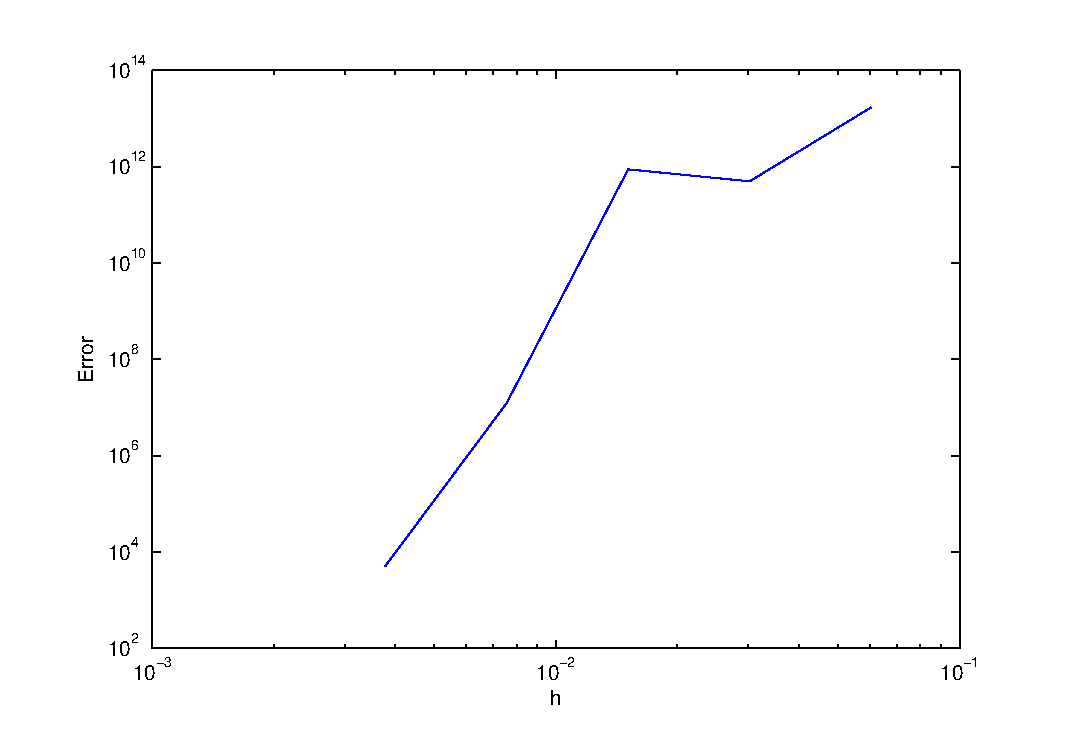
\includegraphics[width=5cm]{e2_l1err_vs_h.eps}}
\subfigure{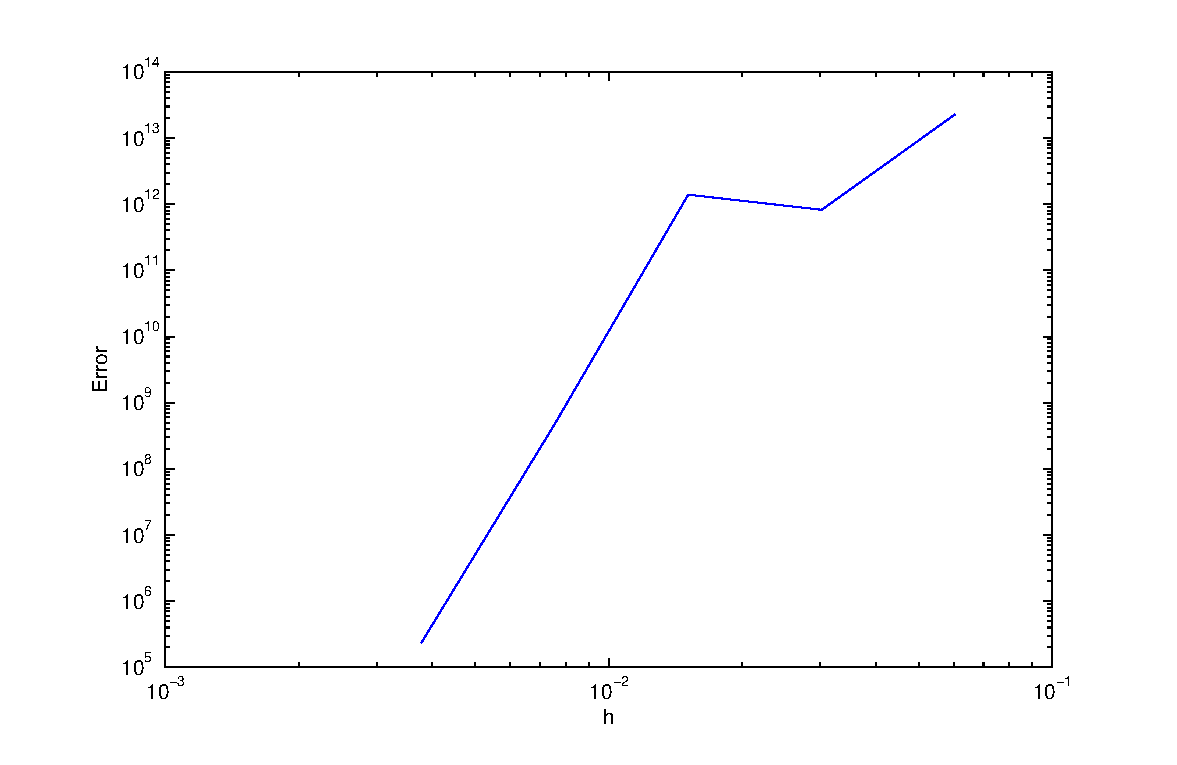
\includegraphics[width=5cm]{e2_l2err_vs_h.eps}}
\caption{Discretization error measured in L1- and L2-norms, depenence on $h$, for $\epsilon=0$.}
\end{figure}

\begin{figure}[!ht]
\centering
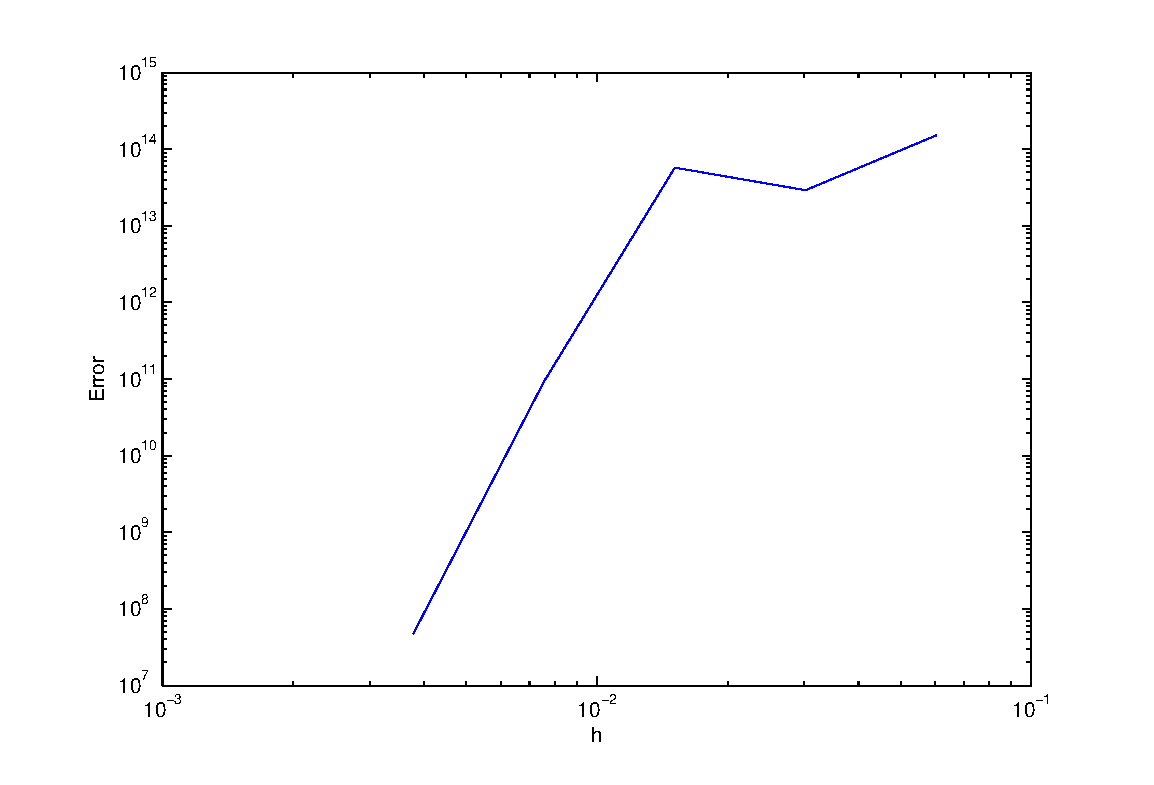
\includegraphics[width=5cm]{e2_linferr_vs_h.eps}
\caption{Discretization error measured in the $\infty$-norm, dependence on $h$, for $\epsilon=0$.}
\end{figure}

\section{Experiment 3}

\[-\Delta u + \nabla\cdot(u\nabla\Psi) = 0\]

We wish to solve the above equation on the unit square $[0,1]^2$. It can be readily verified that
$u=e^\Psi$ solves the equation. We use prescribed Dirichlet boundary data and choose $\Psi$ as
follows:

\[\Psi=\Psi(r)=\frac{1}{1+e^{a(r-1)}}.\]

Here, $r=\sqrt{x^2+y^2}$. For $a\gg1$, $\Psi$ will be close to constant for $r\neq1$, and there
will be a sharp layer of strong convection for $r\approx1$.

\begin{figure}[!ht]
\centering
\subfigure{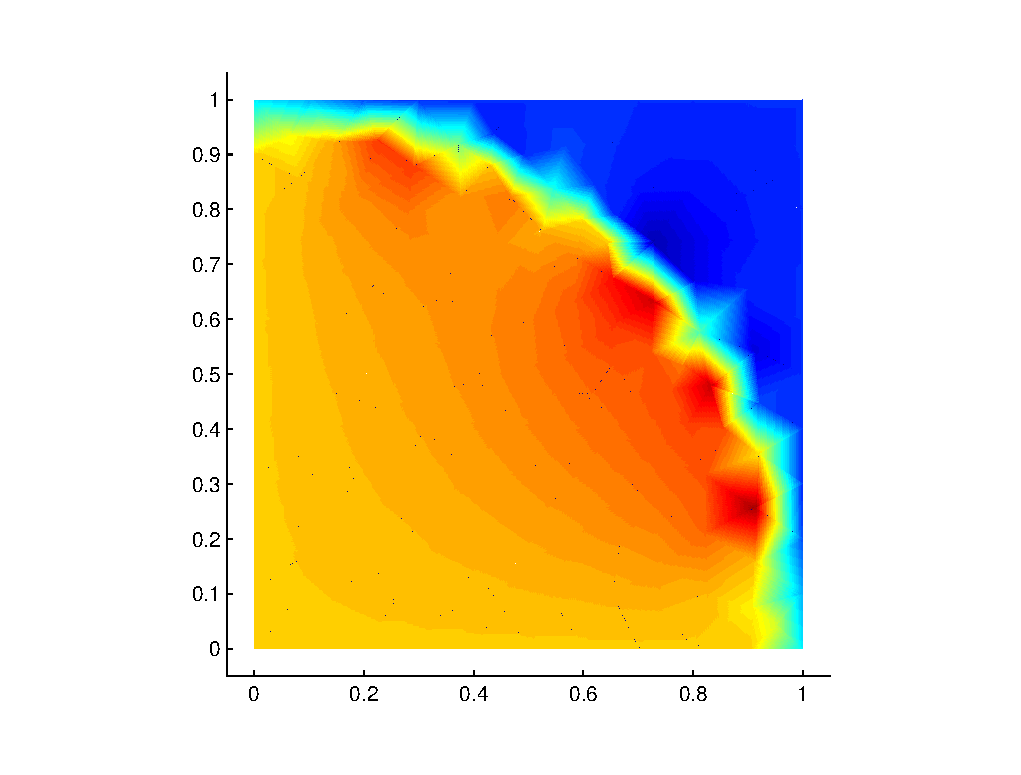
\includegraphics[width=5cm]{e3_sol_h0_a100_top.eps}}
\subfigure{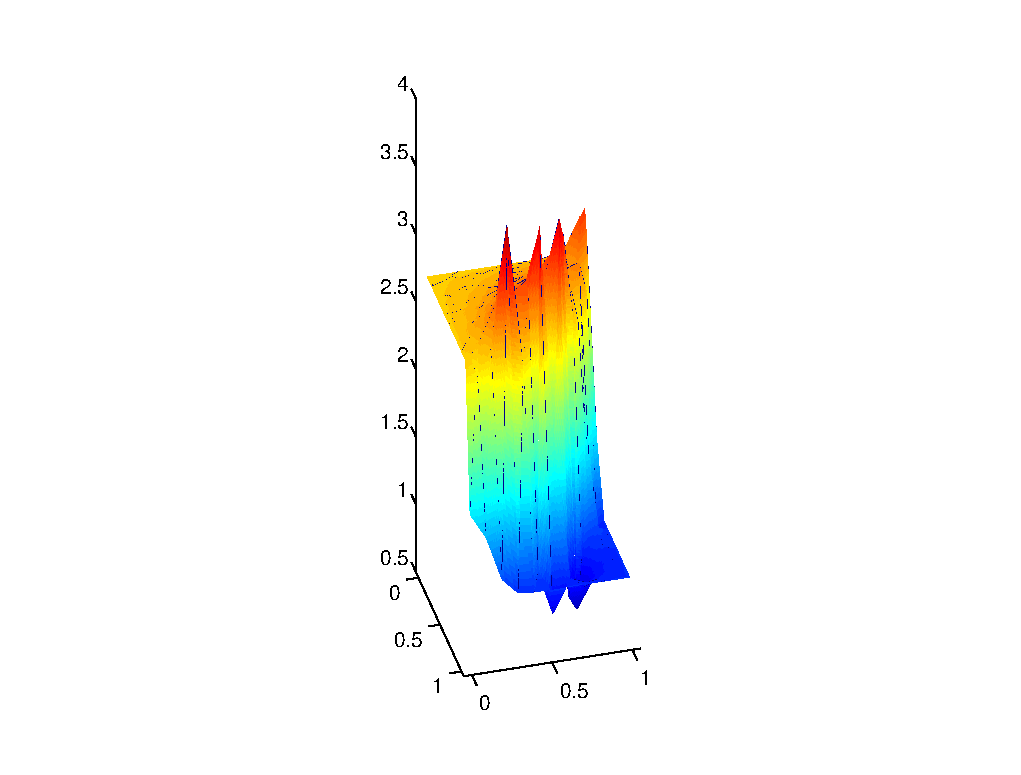
\includegraphics[width=5cm]{e3_sol_h0_a100.eps}}
\caption{Numerical solution for $a=100$, $h=1.21\cdot10^{-1}$.}
\end{figure}

\begin{figure}[!ht]
\centering
\subfigure{\includegraphics[width=5cm]{e3_sol_h4_a100_top.eps}}
\subfigure{\includegraphics[width=5cm]{e3_sol_h4_a100.eps}}
\caption{Numerical solution for $a=100$, $h=7.6\cdot10^{-3}$.}
\end{figure}

\end{document}
